
\section{Source Code}\label{app:source_code}

The source code for the system described in this report can be found at the following address:

\begin{verbatim}
http://github.com/kjellwinblad/HandReco
\end{verbatim}

The source code can be downloaded as a ZIP-archive or cloned using git\footnote{http://git-scm.com/}.

\section{Result Reproduction}\label{app:result_reproduction} 

The test results presented in section~\ref{sec:result} are produced by scripts written in the Jython\footnote{Jython is a version of Python for the Java Virtual Machine (http://www.jython.org/)} programming language. The following steps will run the test scripts:

\begin{enumerate}
 \item Follow the instructions in appendix~\ref{app:source_code} to download the source code for the system.
 \item Follow the instructions in the \verb|README.md| file in the root of the source code directory. These instructions will help you to set up your environment for running the test scripts.
 \item Open a system terminal and execute the following commands (Notice that the path may look different in your system):
 \begin{enumerate}
  \item \verb|cd /path/to/HandReco/src/test|
  \item To run tests for word classifier:
  \item \verb|jython word_classifer_tester.py|
  \item To run tests for character classifier:
  \item \verb|jython character_classifier_tester.py|
 \end{enumerate}
\end{enumerate}

\section{Testing Handwriting Recognition in Graphical User Interface}
%Kjell Describe the GUI for running the HandReco Writer and perhaps some comments on how it works
A graphical user interface (GUI) has been created in order to test the handwriting recognition system in practice. See figure~\ref{fig:hand_reco_writer_screenshot} for a screenshot of the graphical user interface. The following steps can be used to run the GUI:

\begin{enumerate}
 \item Follow the instructions in appendix~\ref{app:result_reproduction} to step 2.
 \item Open a system terminal and execute the following commands (Notice that the path may look different in your system):
 \begin{enumerate}
  \item \verb|cd /path/to/HandReco/src/gui}|
  \item \verb|jython hand_reco_writer.py|
 \end{enumerate}
\end{enumerate}

The GUI can only recognize capital Latin letters. To see which words are available for word corrections click on the \textbf{Info$\Rightarrow$Available Words...} menu item. To input a character, first paint the character in the paint area and then press the \textbf{Write Character} button. To do a space, press the \textbf{Space} button. To do a space and let the word classifier correct the last word, press the \textbf{Space and Correct} button.

    \begin{figure}[htb] 
      \begin{center}
	\leavevmode
	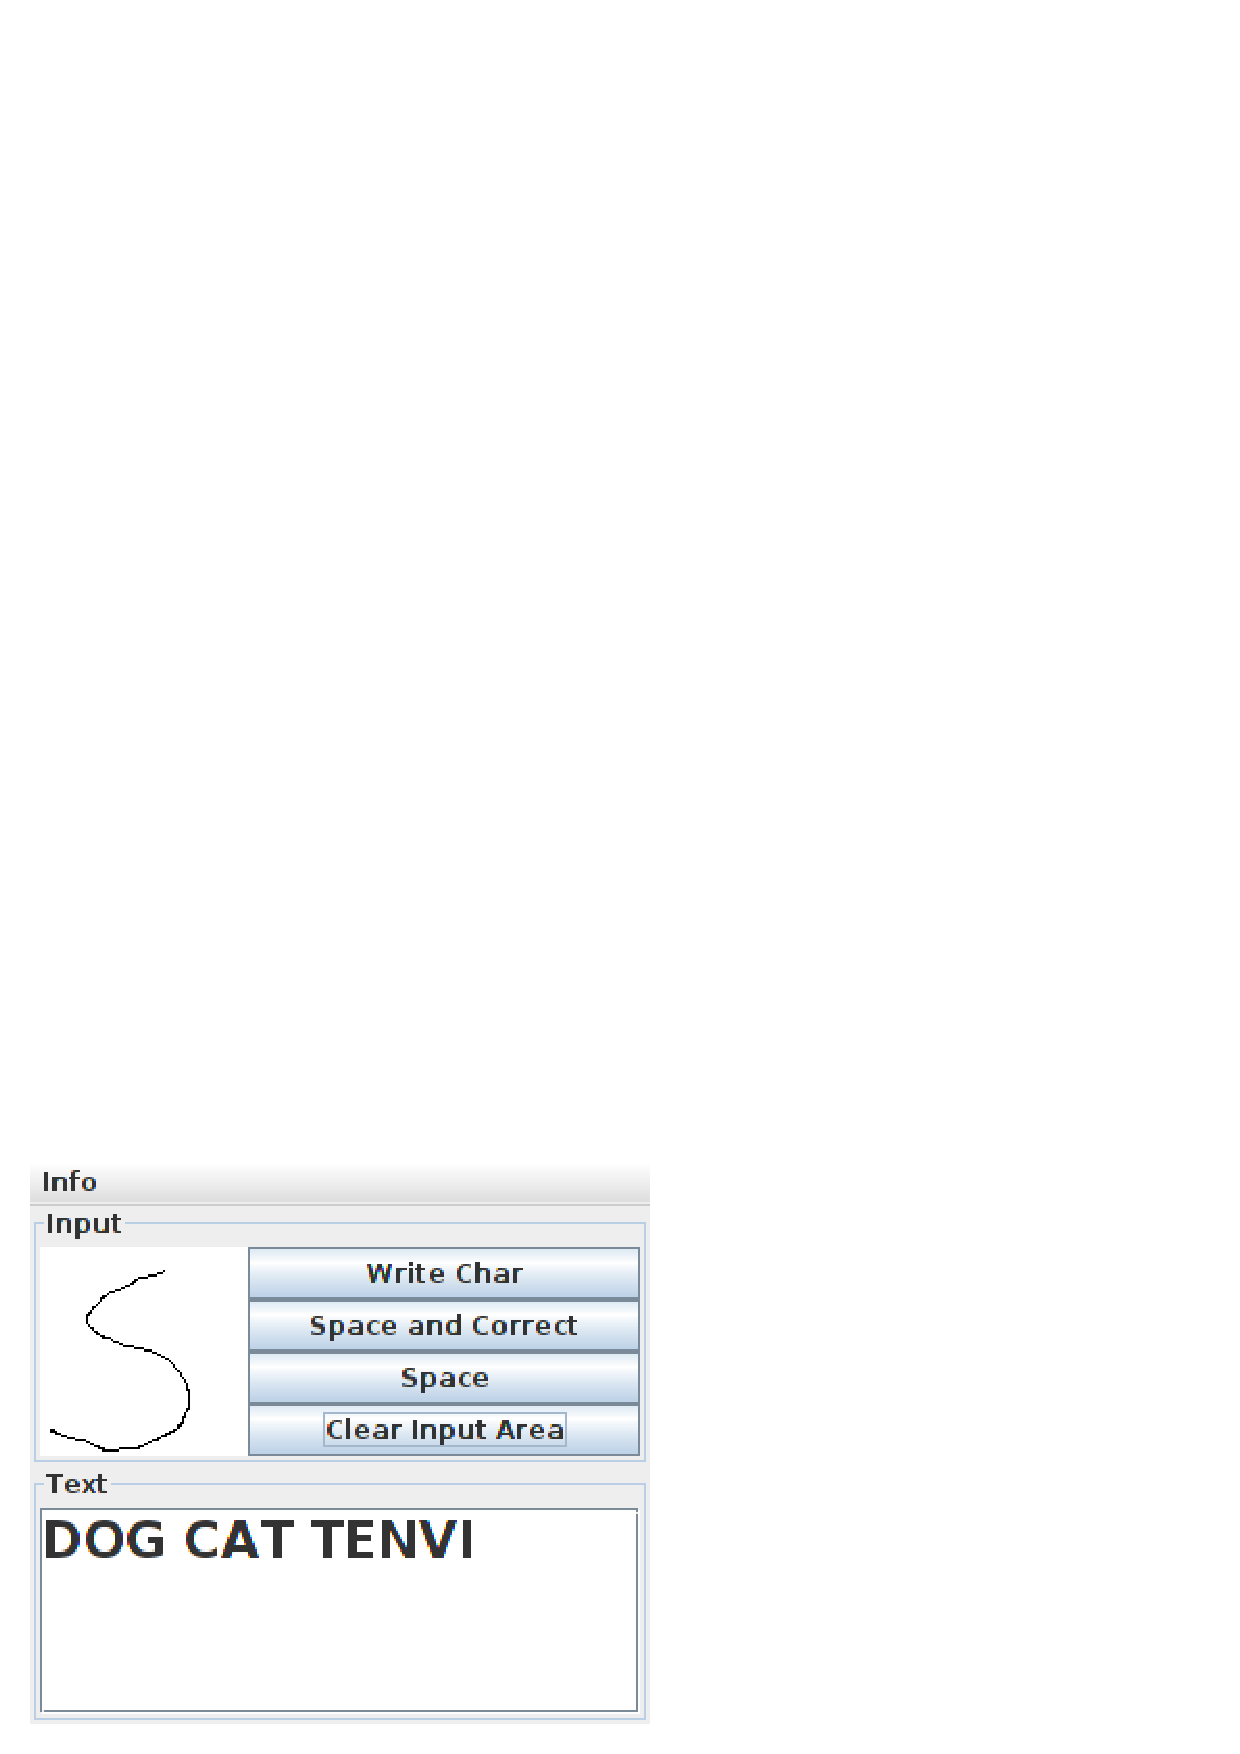
\includegraphics[width=80mm]{Screenshot_HandReco_Writer.png}%width=115mm,height=40mm
      \end{center}
      \caption{Screenshot of HandReco Writer.}
      \label{fig:hand_reco_writer_screenshot}
    \end{figure}
